\documentclass{beamer}
\usepackage{graphicx}
\usepackage{epstopdf}
\usepackage{url}

% Asher's REST tutorial
% Date: 2015

% Title page
\title{RESTful Web Services in Science}
\author{Asher Pasha}
\institute{University of Toronto}
\date{November 5, 2015}

\begin{document}

	\frame{\titlepage}

	\begin{frame}
		\frametitle{CGI Programs}
		\begin{figure}[!htb]
			\centering
			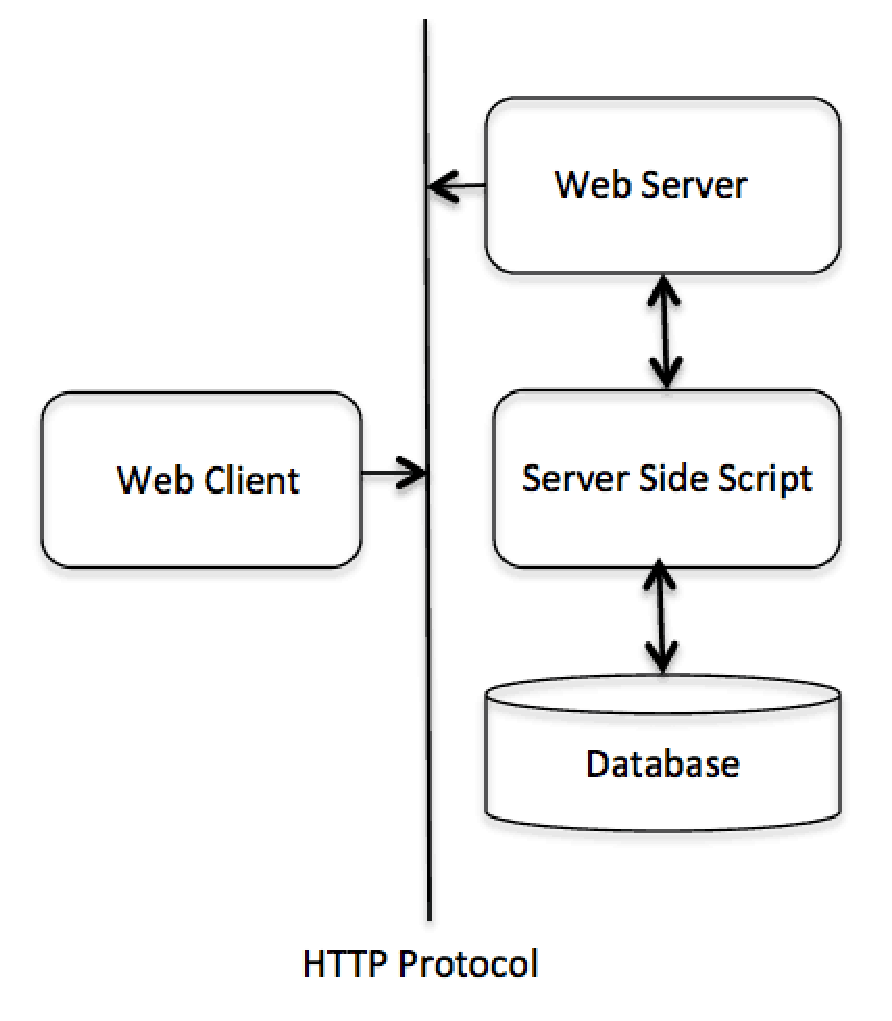
\includegraphics[width=2in]{cgiarch.eps}
			\caption{Perl/Python web program back in the good old days of CGI}
		\end{figure}
		Example: \url{https://bar.utoronto.ca/efp\_arabidopsis/cgi-bin/efpWeb.cgi}
		{\tiny Source: \url{https://www.tutorialspoint.com/perl/perl\_cgi.htm}}
	\end{frame}

	\begin{frame}
		\frametitle{Web 2.0}
		\begin{figure}[!htb]
			\centering
			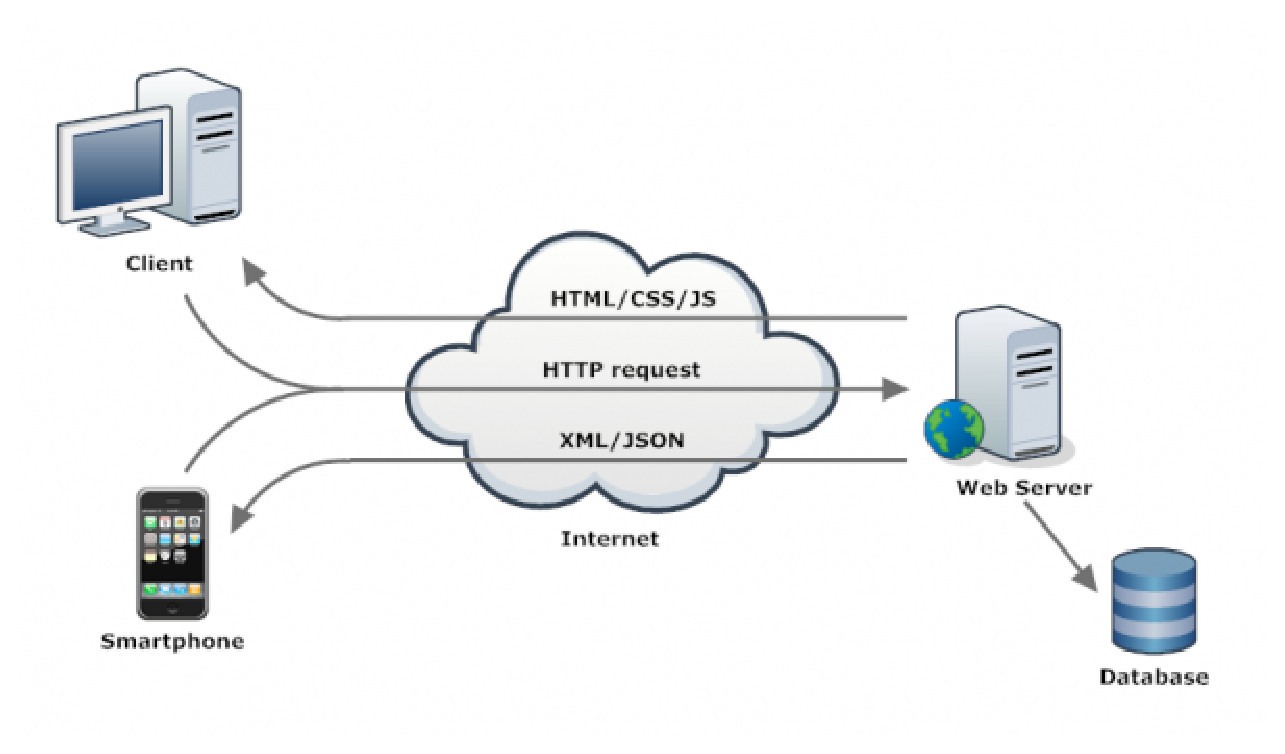
\includegraphics[width=2in]{REST.eps}
			\caption{Modern REpresentational State Transfer}
		\end{figure}
		\begin{itemize}
			\item Input: HTTP GET request
			\item Output: XML, JSON, SVG, png
		\end{itemize}
		{\tiny Source: http://di-side.com/di-side/services/web-solutions/rest-webservice-symfony/}			
	\end{frame}

	\begin{frame}
		\frametitle{AIV: Database and webservice}
		\begin{figure}[!htb]
			\centering
			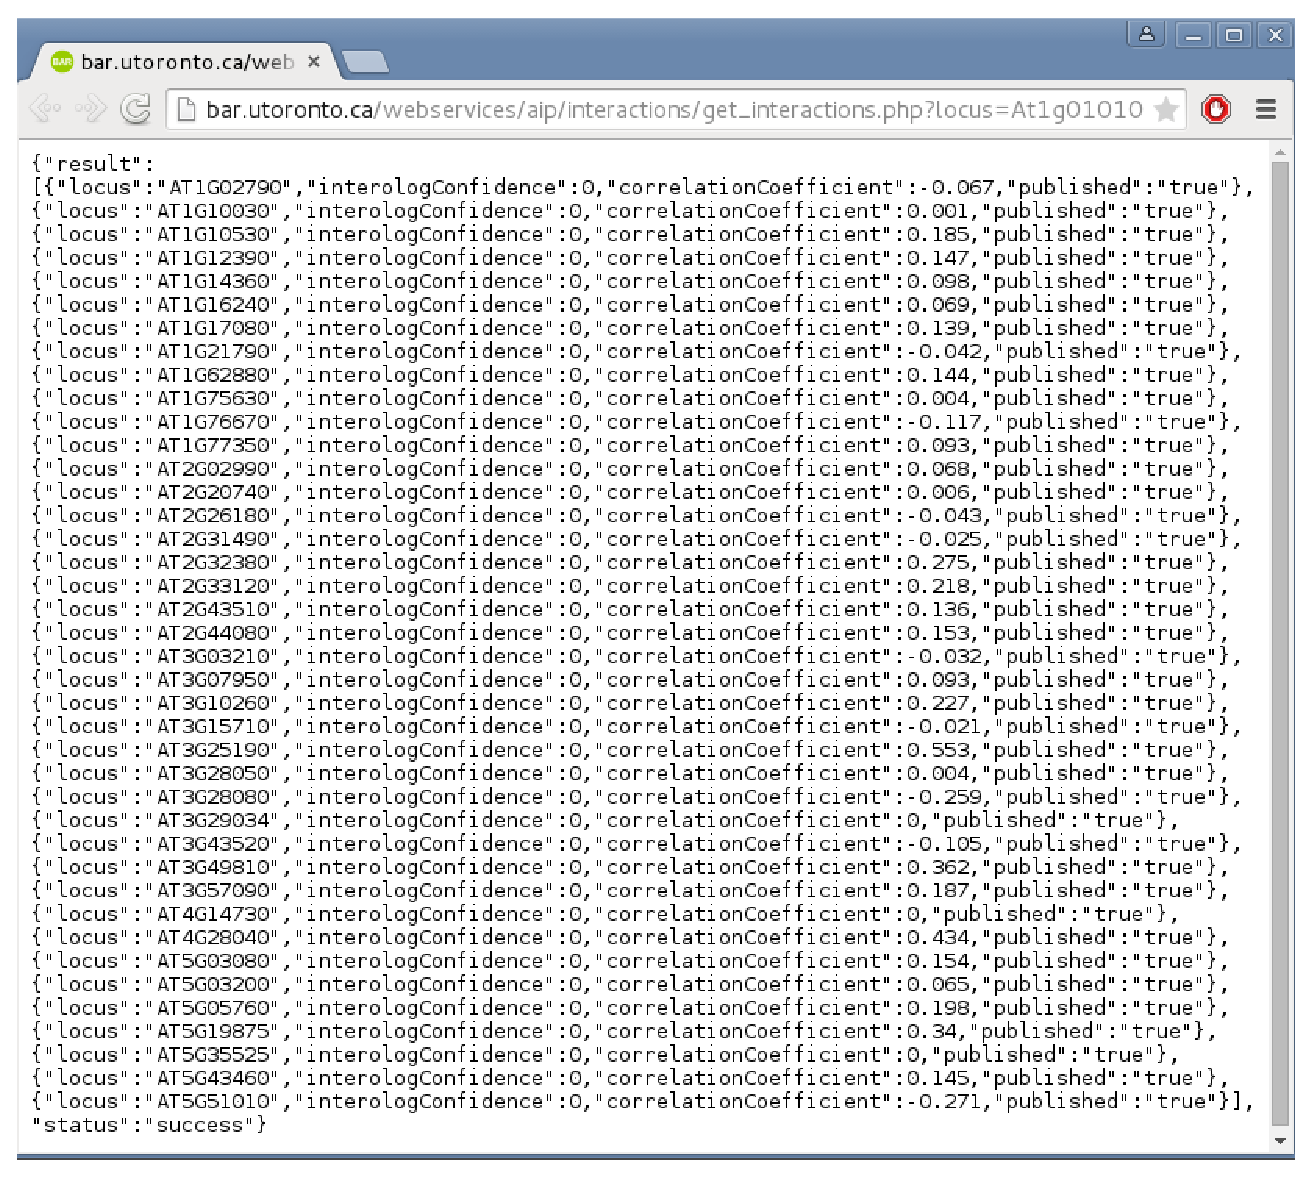
\includegraphics[width=3in]{webservice.eps}
			\caption{The Web Service called for At1g01010}
		\end{figure}
	\end{frame}

	\begin{frame}
		\frametitle{Toy Example of REST}
		\begin{itemize}
			\item All \url{http://services.groupkt.com/country/get/all}
			\item CA \url{http://services.groupkt.com/country/get/iso2code/CA}
			\item CAD \url{http://services.groupkt.com/country/get/iso3code/CAN}
		\end{itemize}
		Python Code Demo
	\end{frame}

	\begin{frame}
		\frametitle{RESTful Web Services}
		Some service providers in Biology
		\begin{itemize}
			\item Reactome \url{http://reactomews.oicr.on.ca:8080/ReactomeRESTfulAPI/ReactomeRESTFulAPI.html}
			\item ATTED-II \url{http://atted.jp/help/API.shtml}
			\item BAR \url{https://bar.utoronto.ca/webservices/}
		\end{itemize}
		Searching and demystifying output
		\begin{itemize}
			\item JSON Lint: \url{http://jsonlint.com/}
			\item Most database websites have REST web services described in API documentation section
		\end{itemize}
	\end{frame}

	\begin{frame}
		\frametitle{Working example}
		\begin{itemize}
			\item TAIR for Plant Biology 
			\item Araport being made by The J. Craig Venter Institute, Texas Advanced Computing Center, and University of Cambridge
			\item \url{https://www.araport.org/}
			\item Community extensible Science Apps
			\item We (BAR at University of Toronto) are also working on Science Apps
		\end{itemize}
	\end{frame}

	% Araport Interactions Viewer
	\begin{frame}
		\frametitle{Science Apps On Araport}
		\begin{itemize}
			\item Web Apps must be written in HTML5/CSS/JavaScript
			\item Araport allows developers to develop fully functional apps in their local development environment and test them on Araport site
			\item Developers can also develop Araport Data Mediator API (ADAMA) adaptors to access web services on 3rd party websites
			\item The ADAMA adaptors (Python clients for RESTful web services) can be called by using Agave API from web apps
		\end{itemize}
		(Krishnakumar V. \textit{et al.}, 2015)
	\end{frame}

	\begin{frame}
		\frametitle{Araport Architecture}
		\begin{figure}[!htb]
			\centering
			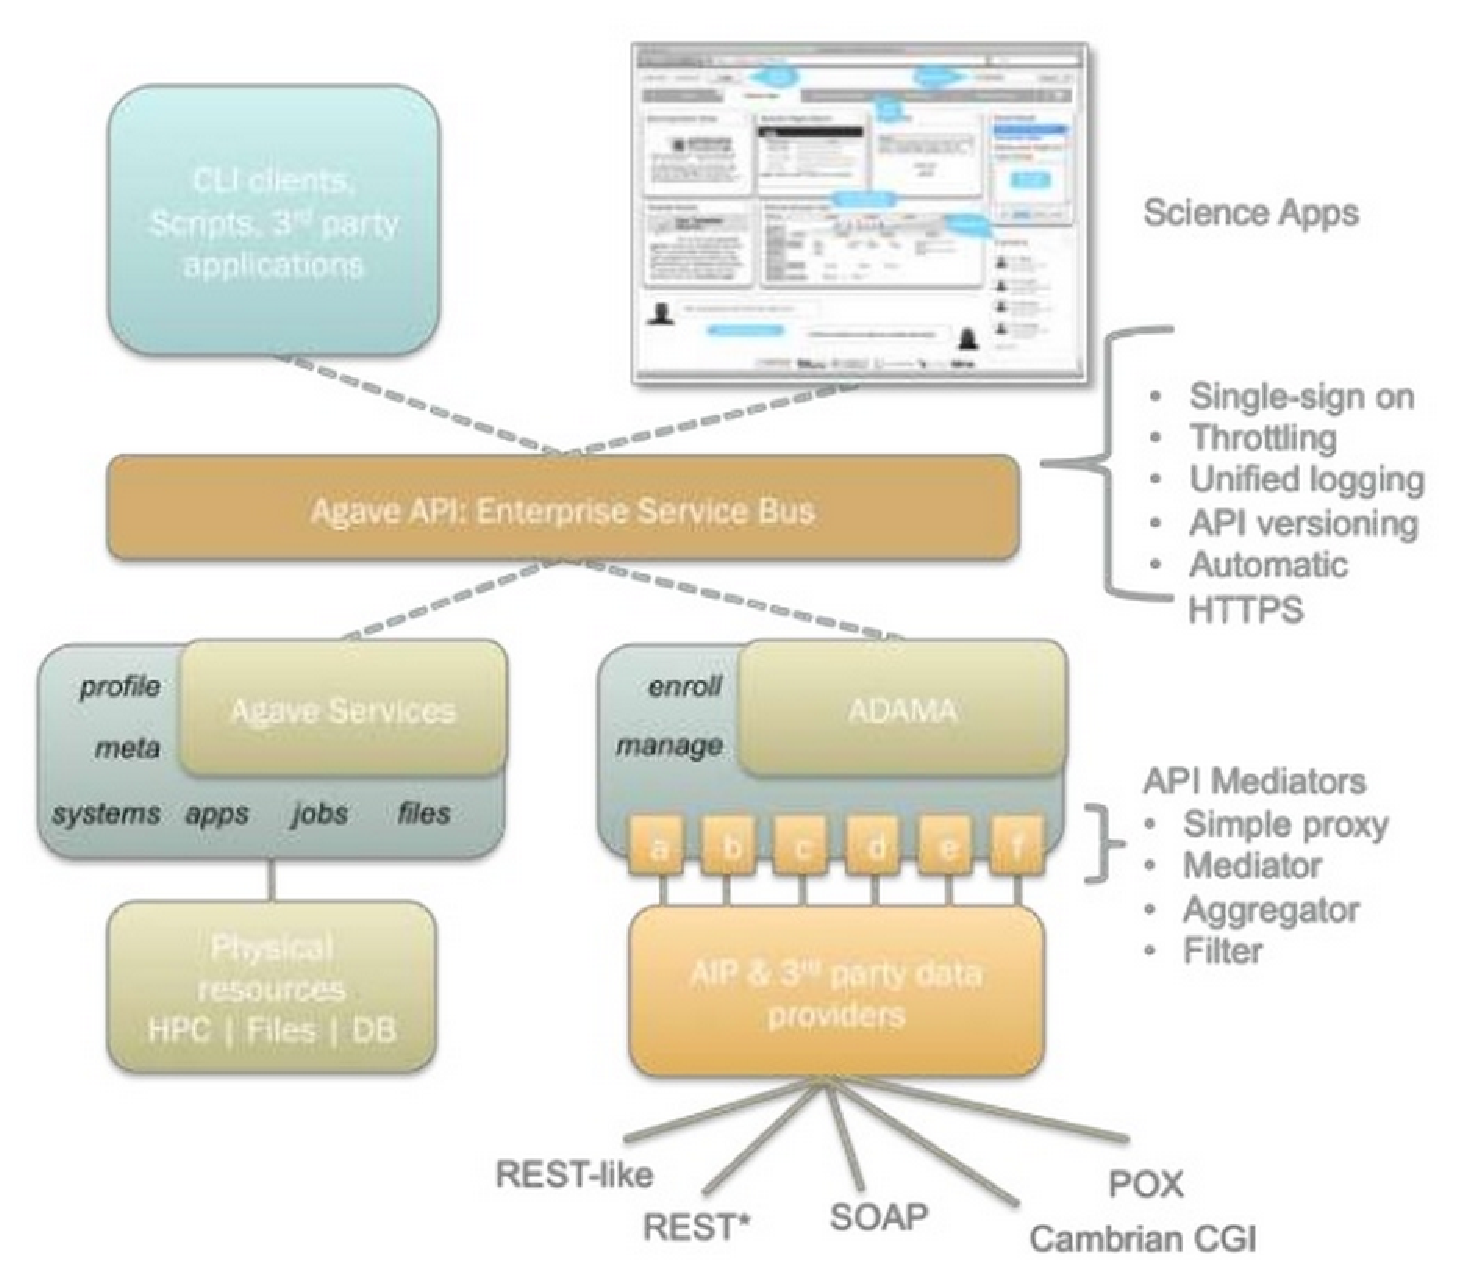
\includegraphics[width=3in]{Araport.eps}
		\end{figure}
		Source: Araport workshop tutorial
	\end{frame}

	\begin{frame}
		\frametitle{Web Application Development Stack}
		The following are used to develop Araport webapps
		\begin{itemize}
			\item Yeoman application generator
			\item Grunt task runner
			\item Bower package manager
			\item npm (node package manager)
			\item OAuth 2.0 for Agave API access
			\item HTML5/CSS/JavaScript
			\item Swagger-js for API documentation
		\end{itemize}
	\end{frame}

	\begin{frame}
		\frametitle{Arabidopsis Interactions Viewer}
		An interactions Viewer was developed for Araport
		\begin{itemize}
			\item Interactions database is on the BAR
			\item RESTful web service gets data from database on the BAR
			\item ADAMA medicator (in Python 2.7 and YAML) on Araport workspace to access the web service from Araport
			\item Interactions displayed using Cytoscape JS plugin
			\item Developed using HTML5/CSS/JavaScript
			\item Hosted on GitHub
			\item Backend:	\url{https://github.com/asherpasha/AIP_interactions_webservice}
			\item Frontend: \url{https://github.com/asherpasha/AIP_interactions_viewer}
		\end{itemize}
		(Geisler-Lee J. \textit{et al.}, 2007)
	\end{frame}

	\begin{frame}
		\frametitle{AIV: Screenshot}
		\begin{figure}[!htb]
			\centering
			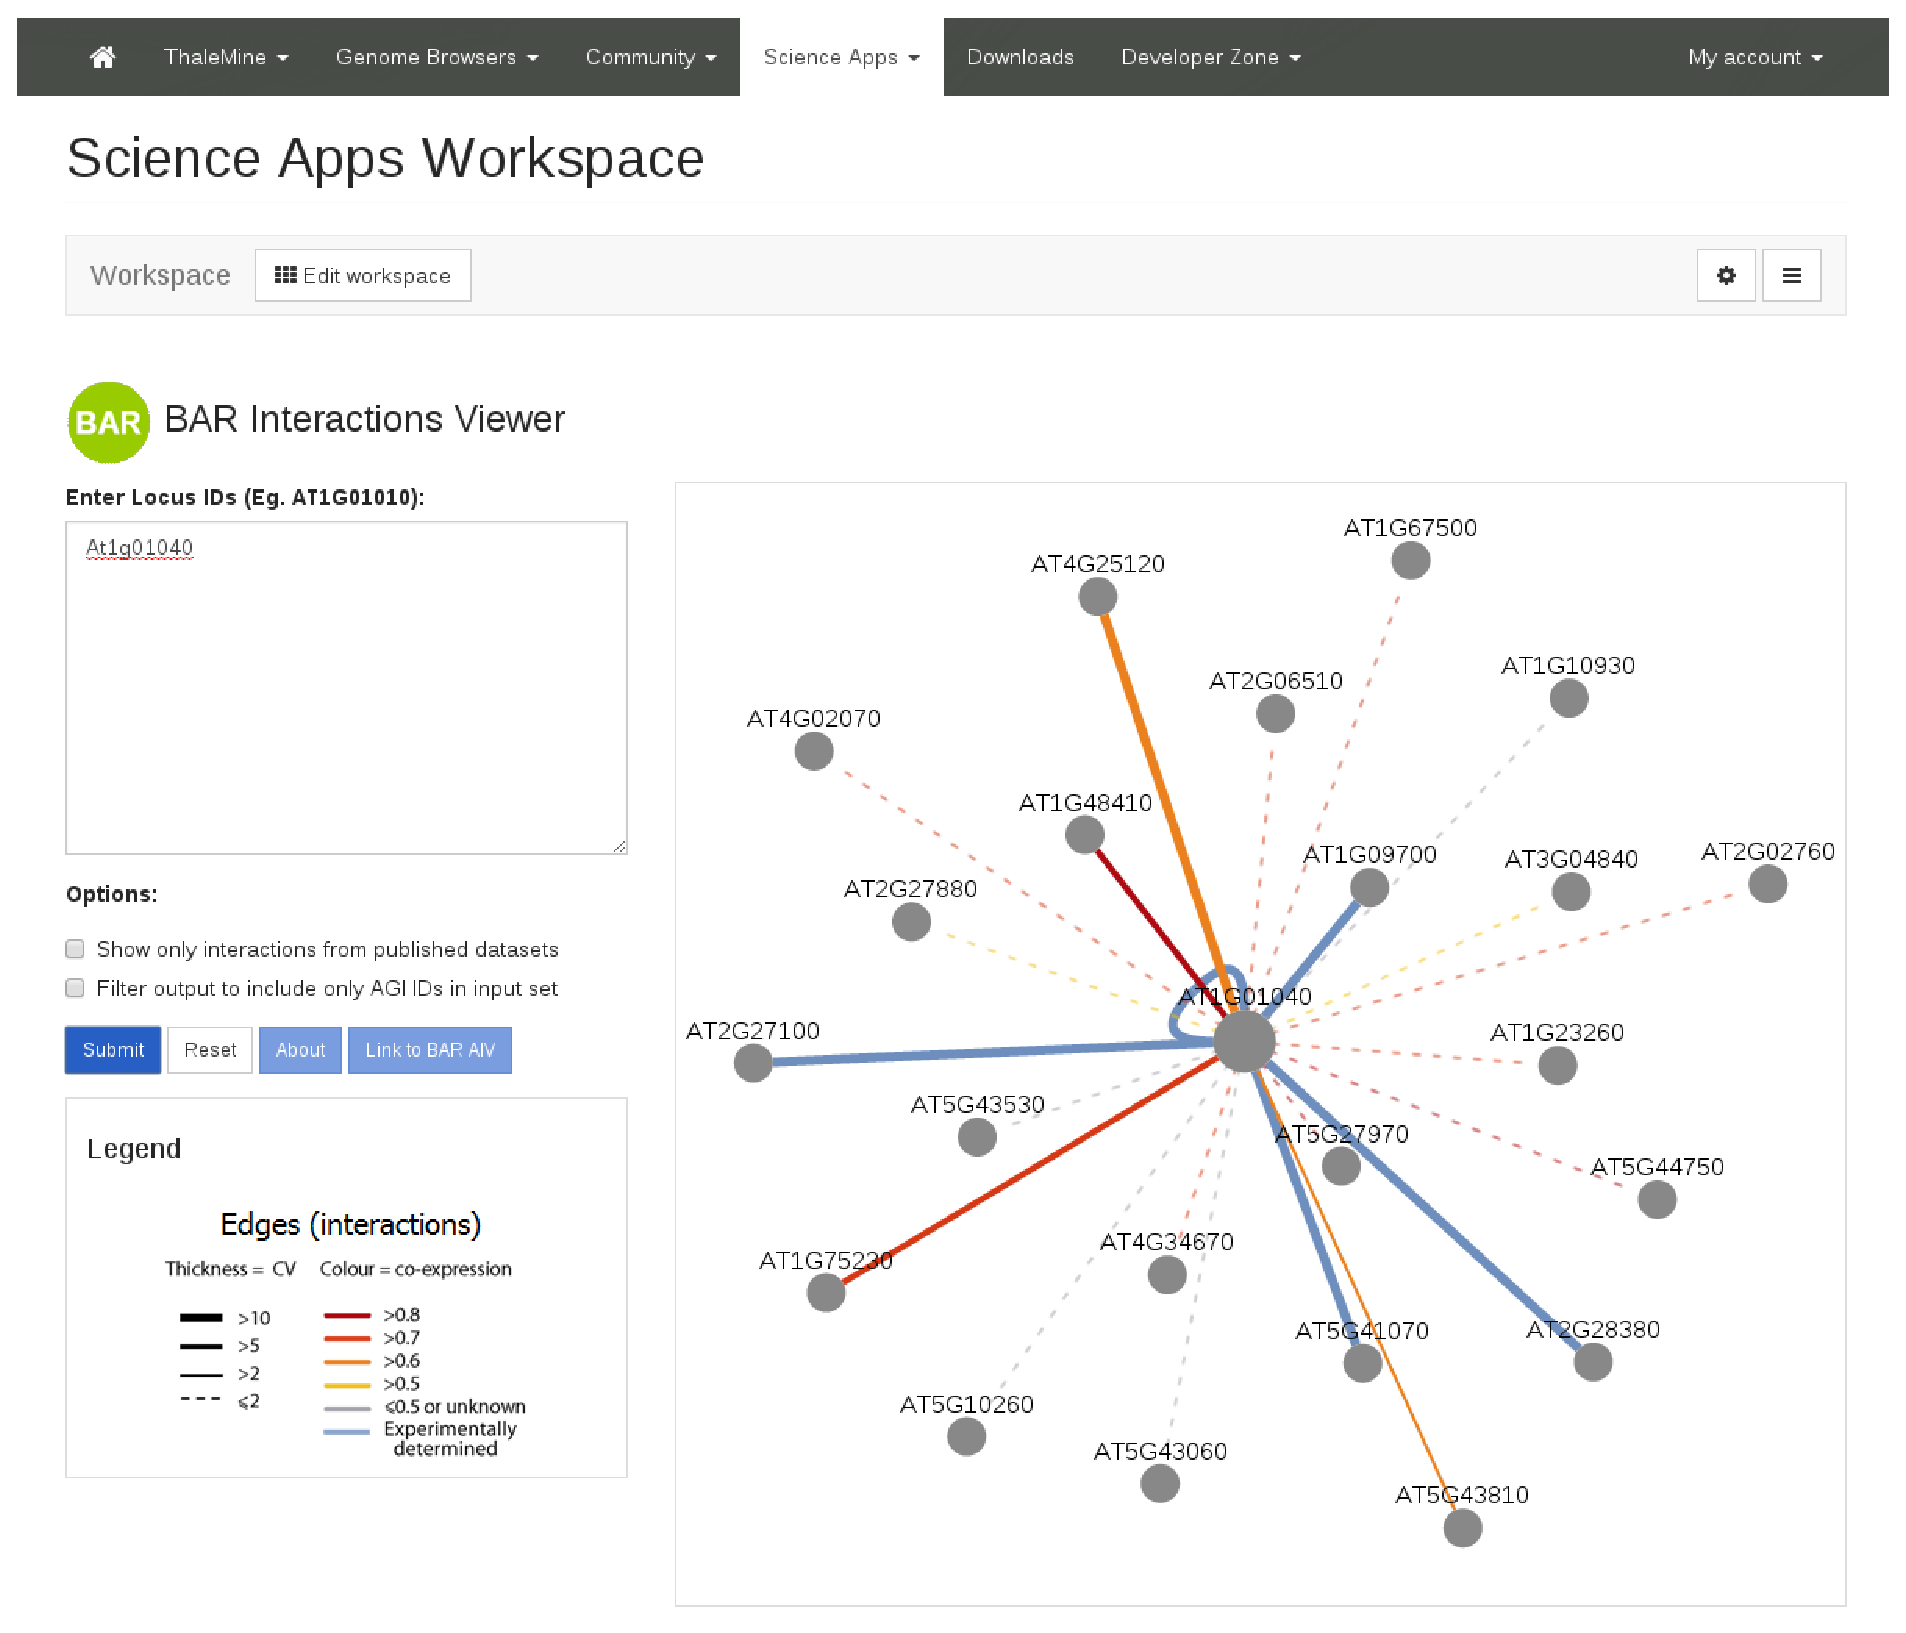
\includegraphics[width=3in]{AIV.eps}
			\caption{Interactions viewer running on Araport}
		\end{figure}

	\end{frame}

	\begin{frame}
		\frametitle{Acknowlegements}
		\begin{columns}[c]
			\column{.5\textwidth}
			Provart Lab and CAGEF
			\begin{itemize}
				\item Prof. Provart
				\item Prof. Guttman
				\item Jamie Waese
				\item Sylva Donaldson
				\item Yunchen Gong
				\item Ryan Austin
				\item Hardeep Nahal
				\item Anna van Weringh
				\item Michael Dong
				\item Matthew Ierullo
				\item Rohan Patel
				\item Nina Wang
				\item Richard Song
			\end{itemize}

			\column{.5\textwidth}
			Araport/JCVI/TACC
			\begin{itemize}
				\item Prof. Chris Town
				\item Prof. Jason Miller
				\item Matt Vaughn
				\item Vivek Krishnakumar
				\item Matt Hanlon
			\end{itemize}
			Others
			\begin{itemize}
				\item U of T Scientific Coders
				\item Joshua Heimbach (Araport workshop team)
			\end{itemize}
			Funding
			\begin{itemize}
				\item Genome Canada
				\item CAGEF
				\item University of Toronto
			\end{itemize}
		\end{columns}
	\end{frame}

\end{document}
